\documentclass[11pt,a4paper]{article}
\usepackage[T1]{fontenc}
\usepackage{lmodern}
\usepackage[margin=2.2cm]{geometry}
\usepackage{amsmath,amssymb,graphicx,booktabs,tabularx,array,float,caption,xcolor}
\usepackage[section]{placeins}
\usepackage{longtable}
\usepackage[numbers,sort&compress]{natbib}
\usepackage[colorlinks=true,linkcolor=blue!45!black,citecolor=blue!45!black,urlcolor=blue!45!black]{hyperref}
\graphicspath{{figures/}}
\captionsetup{font=small,labelfont=bf}
\setlength{\parskip}{3pt}
\makeatletter
\setlength{\@fptop}{0pt}
\setlength{\@fpsep}{14pt}
\setlength{\@fpbot}{0pt plus 1fil}
\makeatother
\renewcommand{\topfraction}{0.95}
\renewcommand{\bottomfraction}{0.95}
\renewcommand{\textfraction}{0.06}
\renewcommand{\floatpagefraction}{0.80}
\setlength{\textfloatsep}{16pt plus 3pt minus 3pt}
\setlength{\floatsep}{14pt plus 3pt minus 3pt}
\setlength{\emergencystretch}{2em}
\renewcommand{\arraystretch}{1.15}
\newcolumntype{Y}{>{\raggedright\arraybackslash}X}
\title{\textbf{Supplementary Methods and Complete Results}\\[0.5em]\large VOLT-KD: Amplitude-Preserving Learning\\for Lightweight Multi-Label ECG Classification}
\author{}
\date{}
\renewcommand{\thesection}{S\arabic{section}}
\begin{document}
\maketitle
\vspace{-2em}
\setcounter{table}{0}\renewcommand{\thetable}{S\arabic{table}}
\setcounter{figure}{0}\renewcommand{\thefigure}{S\arabic{figure}}
\section{Comparator Implementation and Measurement Conditions}
MSCA-Mamba was implemented from its public methodological description\cite{cetintas2026}. Three $12\rightarrow32$ convolutional branches use kernel 7, dilation rates 1/2/4, batch normalization, ReLU, and squeeze-and-excitation with reduction ratio 4. The concatenated 96 channels pass through a $1\times1$ fusion convolution, layer normalization, and a unidirectional Mamba module. Mamba uses state dimension 16, local convolution kernel 4, and expansion factor 2. Global average and maximum pooling feed a $192\rightarrow128\rightarrow64\rightarrow5$ classifier, giving 121,149 parameters. Fusion and classifier widths were chosen to satisfy the parameter constraint. Sequence-block and classifier dropout were set locally to 0.1 and 0.3, respectively.

Local MSCA-Mamba input controls used identical networks and training settings. Millivolt inputs were median-centered, whereas z-score inputs were mean-centered and scaled by their standard deviations. VOLT-KD student noise augmentation used standard deviation 0.01 in the respective input units. ECGFounder test predictions averaged logits from four held-out teachers, each containing approximately 30.69 million parameters. Each student training record received soft labels from its corresponding held-out teacher alone.

Efficiency was measured on NVIDIA GB10, with 500 timed GPU repetitions after warm-up and batch size 256 for throughput. CPU measurements used one thread. Timing covered model forward inference, and storage and memory were reported in MiB. Student deployment measurements excluded the training auxiliary head. Teacher computation belonged to the training-stage cost.


\section{Data Structure and Complete Voltage-Probe Results}
PTB-XL diagnostic superclasses can co-occur, so a recording may carry several positive labels (Figure~\ref{fig:dataset}). Independent binary heads and the multi-label loss allow VOLT-KD to represent these relationships. Voltage probes achieved higher ROC-AUC with millivolt representations on both development data and the test fold (Table~\ref{tab:voltage}). Amplitude-related information was therefore present beyond a single test partition.
\begin{figure}[htbp]
\centering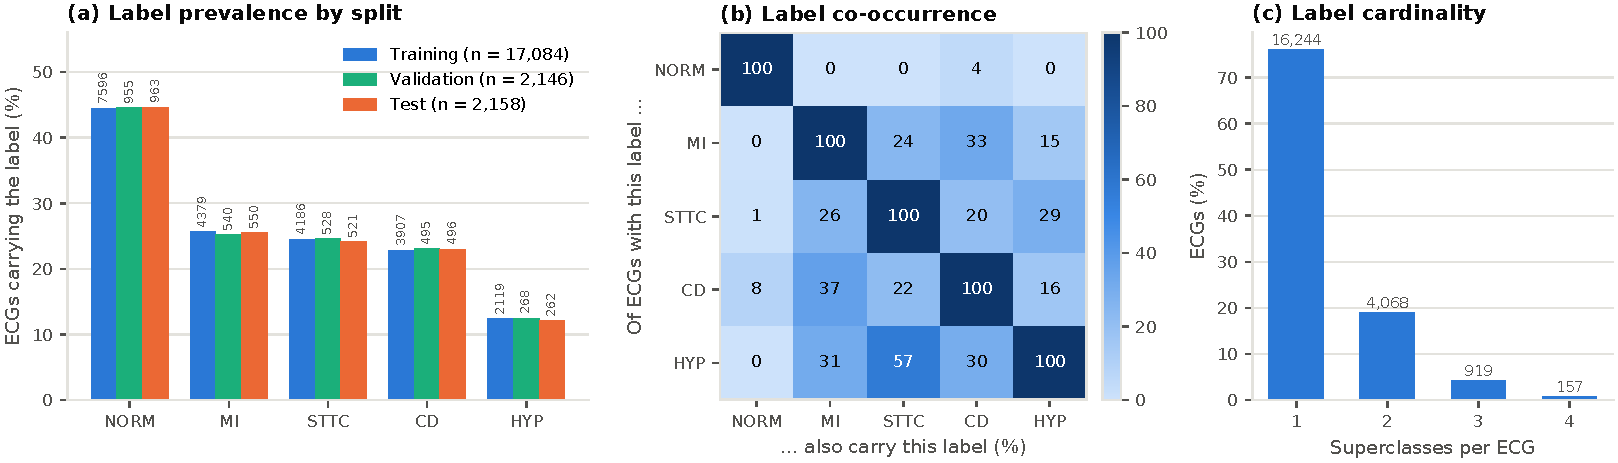
\includegraphics[width=\linewidth,height=0.40\textheight,keepaspectratio]{f01_dataset.pdf}
\caption{Diagnostic superclass distributions, co-occurrence, and label counts. Splits are patient-disjoint, and labels can co-occur.}\label{fig:dataset}
\end{figure}

\begin{table}[htbp]
\centering
\footnotesize
\caption{Training-free voltage-probe ROC-AUC on development data and the test fold. Development data comprise the training and validation folds.}
\label{tab:voltage}
\begin{tabular}{lllrrr}
\toprule
Data & Target & Metric & Positives & mV & z-score \\
\midrule
Test fold & HYP & Sokolow-Lyon & 262 & \textbf{0.786} & 0.527 \\
Test fold & HYP & Cornell & 262 & \textbf{0.702} & 0.582 \\
Test fold & LVH & Sokolow-Lyon & 214 & \textbf{0.876} & 0.591 \\
Test fold & LVH & Cornell & 214 & \textbf{0.745} & 0.614 \\
Development & HYP & Sokolow-Lyon & 2387 & \textbf{0.809} & 0.500 \\
Development & HYP & Cornell & 2387 & \textbf{0.705} & 0.543 \\
Development & LVH & Sokolow-Lyon & 1918 & \textbf{0.894} & 0.573 \\
Development & LVH & Cornell & 1918 & \textbf{0.723} & 0.576 \\
\bottomrule
\end{tabular}
\end{table}
\section{Training and Classwise Prediction Behavior}
Figure~\ref{fig:training} shows five-seed validation trajectories for VOLT-KD and local MSCA-Mamba; all checkpoints were selected using validation data. Classwise ROC, precision--recall curves, and confusion matrices at validation-selected thresholds appear in Figures~\ref{fig:roc}, \ref{fig:pr}, and~\ref{fig:confusion}, respectively. Table~\ref{tab:class} reports six classwise metrics. These results characterize both ranking and threshold decisions, retaining class differences that a single macro metric would obscure.
\begin{figure}[htbp]
\centering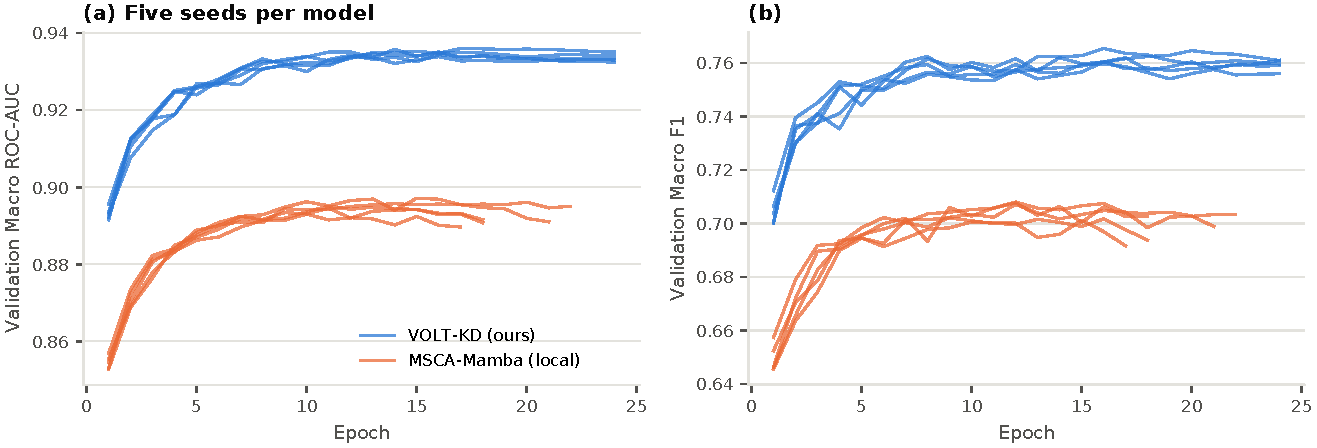
\includegraphics[width=\linewidth,height=0.32\textheight,keepaspectratio]{f04_training_curves.pdf}
\caption{Validation macro ROC-AUC and macro F1 trajectories for complete VOLT-KD and local MSCA-Mamba, each trained with five random seeds.}\label{fig:training}
\end{figure}

\begin{table}[htbp]
\centering\footnotesize
\setlength{\tabcolsep}{3pt}
\caption{Classwise results of complete VOLT-KD as five-seed means and standard deviations. Bold indicates the highest mean among the five classes in each column.}\label{tab:class}
\begin{tabularx}{\linewidth}{Yrrrrrr}
\toprule
Class & ROC-AUC & AP & F1 & Precision & Recall & Specificity \\
\midrule
NORM & $\boldsymbol{0.951\pm0.001}$ & $\boldsymbol{0.932\pm0.002}$ & $\boldsymbol{0.864\pm0.004}$ & $0.801\pm0.016$ & $\boldsymbol{0.938\pm0.012}$ & $0.812\pm0.021$ \\
MI & $0.937\pm0.002$ & $0.860\pm0.005$ & $0.768\pm0.004$ & $0.737\pm0.017$ & $0.801\pm0.023$ & $0.902\pm0.012$ \\
STTC & $0.942\pm0.002$ & $0.837\pm0.006$ & $0.779\pm0.004$ & $0.741\pm0.028$ & $0.823\pm0.030$ & $0.908\pm0.016$ \\
CD & $0.925\pm0.003$ & $0.859\pm0.004$ & $0.768\pm0.008$ & $\boldsymbol{0.835\pm0.017}$ & $0.712\pm0.023$ & $\boldsymbol{0.958\pm0.006}$ \\
HYP & $0.895\pm0.002$ & $0.650\pm0.011$ & $0.592\pm0.008$ & $0.575\pm0.054$ & $0.619\pm0.065$ & $0.935\pm0.020$ \\
\bottomrule
\end{tabularx}

\end{table}

\begin{figure}[htbp]
\centering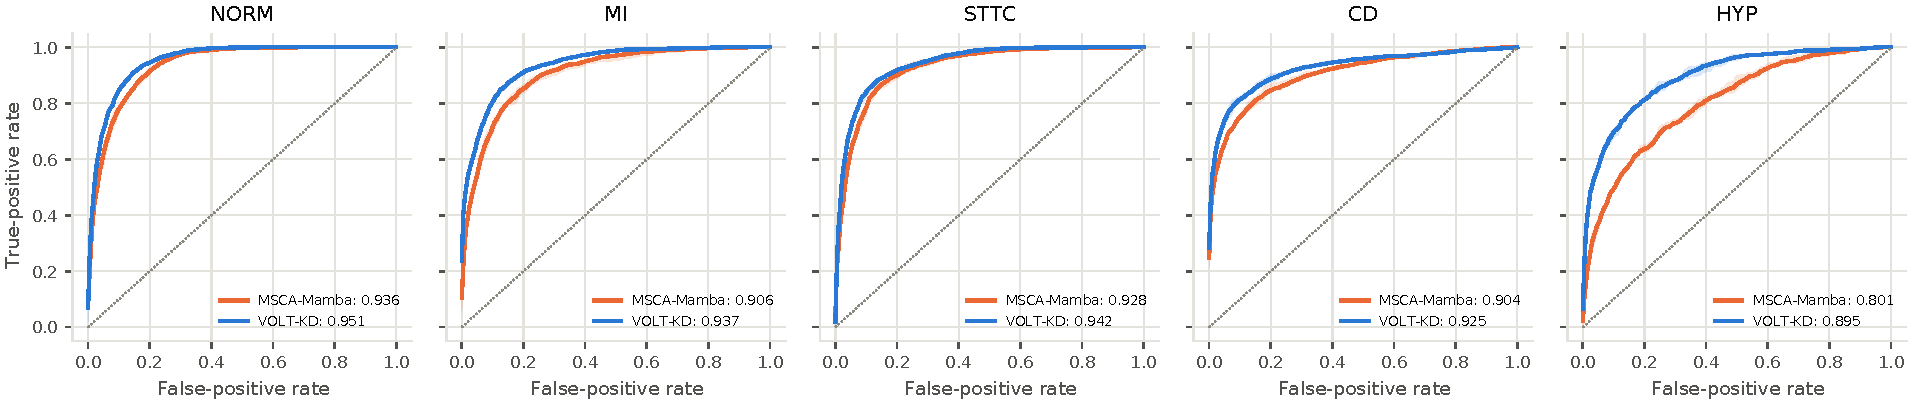
\includegraphics[width=\linewidth,height=0.33\textheight,keepaspectratio]{f08_roc.pdf}
\caption{Classwise ROC curves for complete VOLT-KD and local MSCA-Mamba. Solid lines are five-seed means, and shaded regions span the individual-run curves.}\label{fig:roc}
\end{figure}

\begin{figure}[htbp]
\centering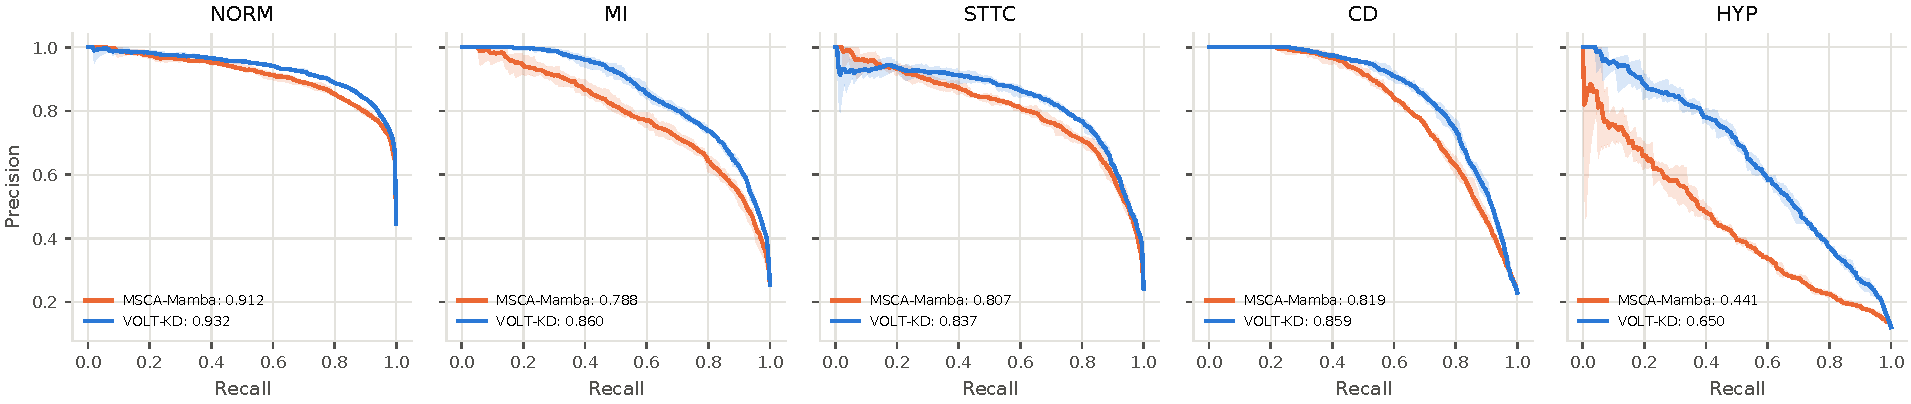
\includegraphics[width=\linewidth,height=0.33\textheight,keepaspectratio]{f09_pr.pdf}
\caption{Classwise precision--recall curves for complete VOLT-KD and local MSCA-Mamba.}\label{fig:pr}
\end{figure}

\begin{figure}[htbp]
\centering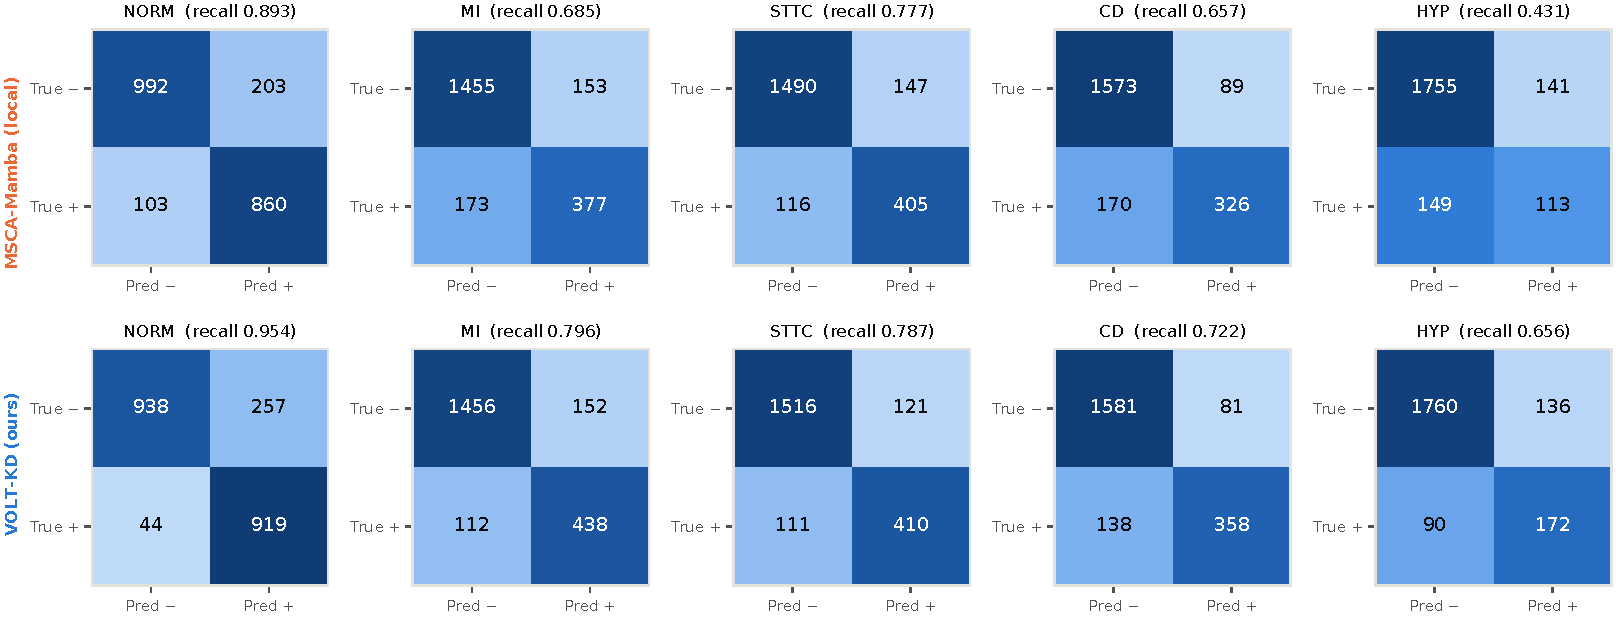
\includegraphics[width=\linewidth,height=0.51\textheight,keepaspectratio]{f10_confusion.pdf}
\caption{Seed-42 binary confusion matrices for local MSCA-Mamba and VOLT-KD. Each class uses its validation-selected threshold.}\label{fig:confusion}
\end{figure}

\section{Additional Literature and Paired-Seed Comparisons}
All 45 mean differences between VOLT-KD and the nine published MSCA-Mamba configurations were positive (Figure~\ref{fig:vsall}). Comparators span convolutional, recurrent, state-space, and attention architectures, supporting higher aggregate performance within this compact-model set. Intervals were approximated from reported standard deviations and describe seed-run summaries. Published and local case-level predictions were not pooled.
\begin{figure}[htbp]
\centering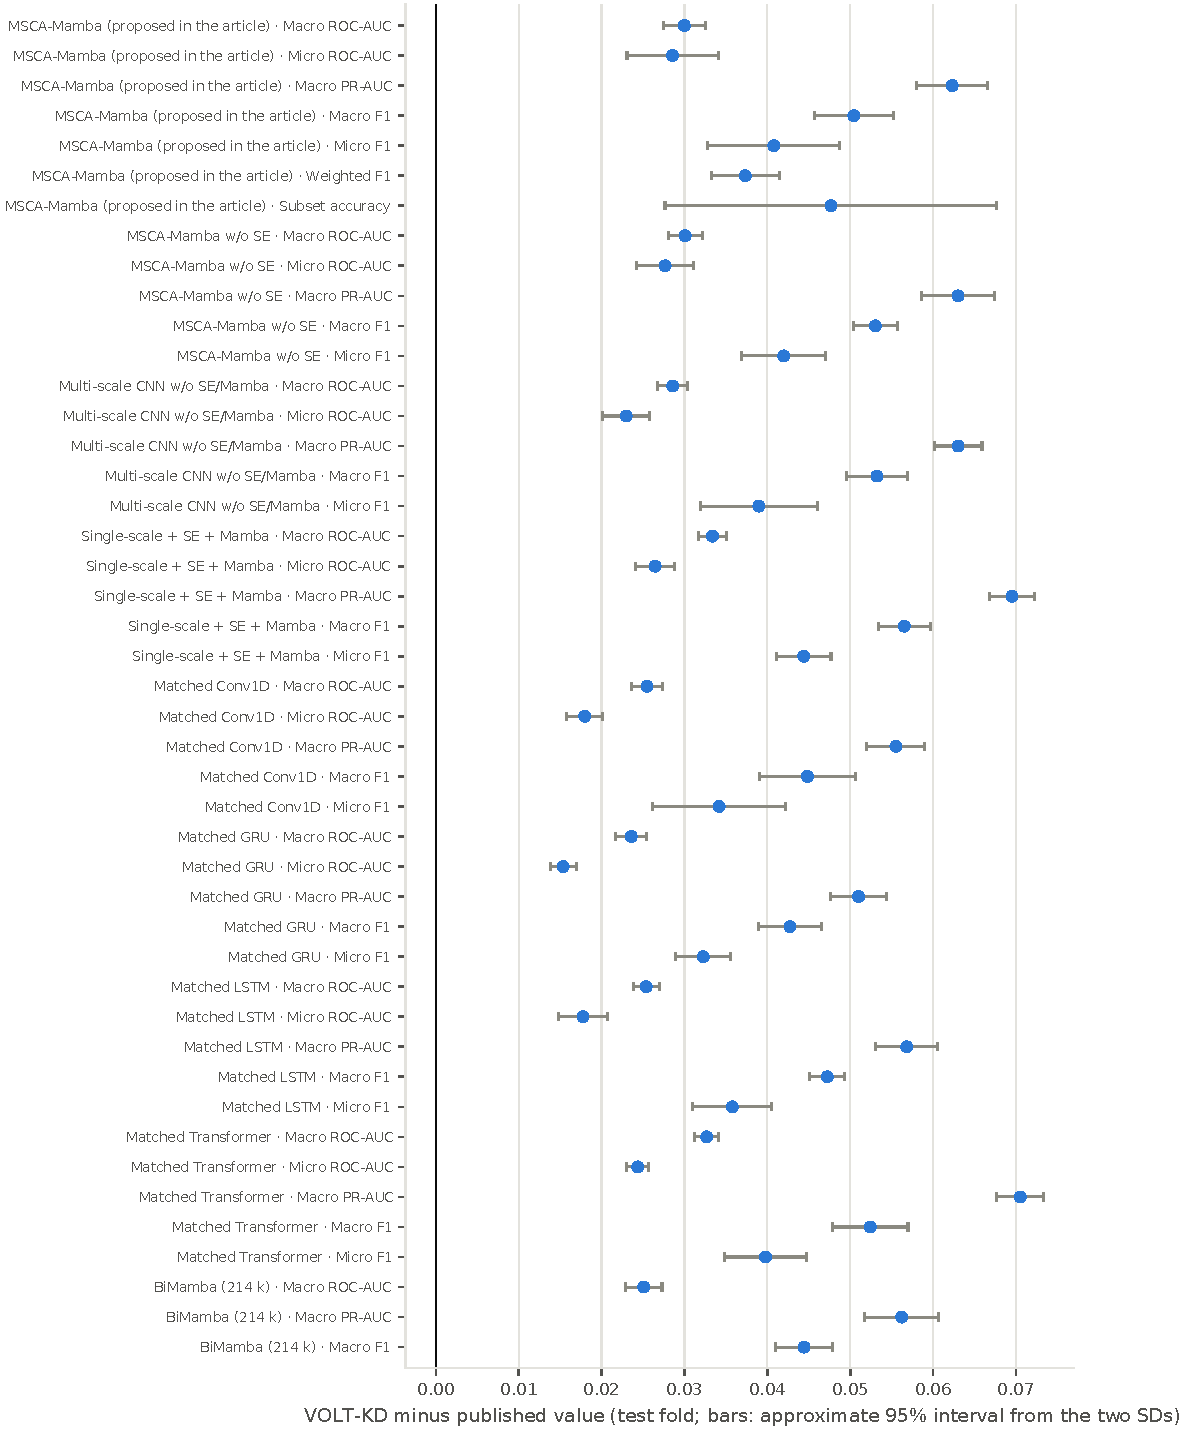
\includegraphics[width=\linewidth,height=0.86\textheight,keepaspectratio]{f06_vs_published.pdf}
\caption{Differences from 45 reported means across nine configurations in the MSCA-Mamba paper\cite{cetintas2026}. Matched metrics are compared; points are VOLT-KD minus published values, with approximate intervals constructed from reported standard deviations.}\label{fig:vsall}
\end{figure}

Table~\ref{tab:paired_full} separately estimates uncertainty from training randomness and test-sample variation. Paired-seed $t$ intervals use metric differences for common seeds, whereas recording-level bootstrap intervals use 1,000 test-record resamples. Distillation increased macro F1 by 0.0043 beyond subclass supervision, with a seed interval of [0.0022, 0.0064] and a recording interval of [$-0.0012$, 0.0100]. These results support an F1 gain across repeated training on the fixed test set, while its sample-level increment varies with resampling. Bootstrap tests also report Holm-adjusted results.
\begin{table}[htbp]
\centering\footnotesize
\caption{Paired results for complete VOLT-KD minus local comparator configurations. Except MSCA-Mamba, all comparators are VOLT-KD backbone ablations. AUC, AP, and F1 are macro-averaged.}\label{tab:paired_full}
\begin{tabularx}{\linewidth}{Ylrrrr}
\toprule
Comparator & Metric & Difference & 95\% Seed interval & 95\% Record interval & $p_{\mathrm{Holm}}$ \\
\midrule
MSCA-Mamba (local) & AUC & +0.0348 & [+0.0328, +0.0368] & [+0.0301, +0.0396] & 0.091 \\
MSCA-Mamba (local) & AP & +0.0738 & [+0.0695, +0.0782] & [+0.0624, +0.0844] & 0.091 \\
MSCA-Mamba (local) & F1 & +0.0602 & [+0.0568, +0.0635] & [+0.0506, +0.0693] & 0.091 \\
Superclass only, z-score & AUC & +0.0192 & [+0.0170, +0.0214] & [+0.0158, +0.0229] & 0.091 \\
Superclass only, z-score & AP & +0.0480 & [+0.0439, +0.0521] & [+0.0376, +0.0572] & 0.091 \\
Superclass only, z-score & F1 & +0.0353 & [+0.0310, +0.0396] & [+0.0279, +0.0431] & 0.091 \\
Superclass only, mV & AUC & +0.0020 & [+0.0012, +0.0029] & [+0.0002, +0.0037] & 1.000 \\
Superclass only, mV & AP & +0.0036 & [+0.0002, +0.0071] & [-0.0013, +0.0081] & 1.000 \\
Superclass only, mV & F1 & +0.0058 & [+0.0034, +0.0082] & [+0.0002, +0.0110] & 1.000 \\
Superclass + subclass & AUC & +0.0017 & [-0.0003, +0.0038] & [+0.0001, +0.0032] & 1.000 \\
Superclass + subclass & AP & +0.0034 & [-0.0017, +0.0085] & [-0.0009, +0.0072] & 1.000 \\
Superclass + subclass & F1 & +0.0043 & [+0.0022, +0.0064] & [-0.0012, +0.0100] & 1.000 \\
Complete supervision z-score & AUC & +0.0119 & [+0.0103, +0.0134] & [+0.0089, +0.0151] & 0.091 \\
Complete supervision z-score & AP & +0.0325 & [+0.0279, +0.0372] & [+0.0230, +0.0415] & 0.091 \\
Complete supervision z-score & F1 & +0.0259 & [+0.0232, +0.0286] & [+0.0186, +0.0331] & 0.091 \\
No subclass targets & AUC & -0.0001 & [-0.0021, +0.0019] & [-0.0011, +0.0008] & 1.000 \\
No subclass targets & AP & -0.0000 & [-0.0027, +0.0027] & [-0.0024, +0.0025] & 1.000 \\
No subclass targets & F1 & +0.0024 & [-0.0013, +0.0061] & [-0.0018, +0.0061] & 1.000 \\
In-sample teacher & AUC & -0.0006 & [-0.0012, -0.0001] & [-0.0019, +0.0004] & 1.000 \\
In-sample teacher & AP & -0.0008 & [-0.0032, +0.0017] & [-0.0039, +0.0018] & 1.000 \\
In-sample teacher & F1 & -0.0018 & [-0.0079, +0.0043] & [-0.0060, +0.0018] & 1.000 \\
noisy-OR head & AUC & -0.0008 & [-0.0016, +0.0000] & [-0.0021, +0.0005] & 1.000 \\
noisy-OR head & AP & -0.0019 & [-0.0137, +0.0099] & [-0.0051, +0.0015] & 1.000 \\
noisy-OR head & F1 & +0.0008 & [-0.0039, +0.0055] & [-0.0040, +0.0063] & 1.000 \\
No GRU & AUC & -0.0001 & [-0.0007, +0.0005] & [-0.0014, +0.0013] & 1.000 \\
No GRU & AP & -0.0019 & [-0.0045, +0.0006] & [-0.0051, +0.0011] & 1.000 \\
No GRU & F1 & +0.0004 & [-0.0053, +0.0061] & [-0.0055, +0.0056] & 1.000 \\
Half-width student & AUC & +0.0004 & [-0.0039, +0.0048] & [-0.0008, +0.0017] & 1.000 \\
Half-width student & AP & -0.0016 & [-0.0188, +0.0157] & [-0.0052, +0.0016] & 1.000 \\
Half-width student & F1 & -0.0039 & [-0.0137, +0.0059] & [-0.0092, +0.0011] & 1.000 \\
\bottomrule
\end{tabularx}

\end{table}

The noisy-OR, no-GRU, and half-width VOLT-KD variants use three common seeds; all other configurations use five common seeds. Bootstrap resampling operates on recordings without clustering repeated recordings from the same patient. Paired analyses are exploratory effect estimates.
\section{Complete Subclass and Subgroup Results}
Table~\ref{tab:subclass} reports parent-class detection rates for twenty-one diagnostic subclasses. Improvements for LVH, AMI, IMI, IRBBB, and AVB connect complete VOLT-KD's multi-label gains to specific diagnostic morphologies. Differences in subclass sample sizes and outcomes are retained. Demographic, device, and recording-condition subgroups use the same test fold (Table~\ref{tab:subgroup}), with intervals from 300 within-group recording resamples. All test records carry manually validated labels.
\begin{table}[htbp]
\centering\footnotesize
\caption{Parent-class detection rates for complete VOLT-KD and local MSCA-Mamba among diagnostic-subclass records. Subclasses contain at least five recordings; values are five-seed means. Differences use unrounded results.}\label{tab:subclass}
\begin{tabularx}{\linewidth}{Ylrrrr}
\toprule
Parent & Subclass & Records & Local comparator & VOLT-KD & Difference \\
\midrule
CD & LAFB/LPFB & 179 & \textbf{0.834} & 0.829 & -0.004 \\
CD & IRBBB & 112 & 0.714 & \textbf{0.805} & +0.091 \\
CD & AVB & 82 & 0.527 & \textbf{0.644} & +0.117 \\
CD & IVCD & 79 & \textbf{0.327} & 0.289 & -0.038 \\
CD & CLBBB & 54 & \textbf{0.993} & 0.989 & -0.004 \\
CD & CRBBB & 54 & \textbf{1.000} & \textbf{1.000} & +0.000 \\
CD & ILBBB & 8 & \textbf{0.850} & 0.750 & -0.100 \\
CD & WPW & 8 & \textbf{0.500} & 0.450 & -0.050 \\
HYP & LVH & 214 & 0.595 & \textbf{0.721} & +0.125 \\
HYP & LAO/LAE & 42 & 0.310 & \textbf{0.362} & +0.052 \\
HYP & RVH & 12 & 0.133 & \textbf{0.250} & +0.117 \\
HYP & RAO/RAE & 10 & 0.120 & \textbf{0.160} & +0.040 \\
MI & IMI & 327 & 0.765 & \textbf{0.826} & +0.061 \\
MI & AMI & 306 & 0.801 & \textbf{0.854} & +0.054 \\
MI & LMI & 20 & \textbf{0.380} & 0.360 & -0.020 \\
NORM & NORM & 963 & 0.899 & \textbf{0.938} & +0.040 \\
STTC & STTC & 222 & 0.765 & \textbf{0.766} & +0.001 \\
STTC & ISC & 128 & 0.925 & \textbf{0.953} & +0.028 \\
STTC & ISCA & 93 & 0.832 & \textbf{0.869} & +0.037 \\
STTC & NST & 77 & 0.779 & \textbf{0.803} & +0.023 \\
STTC & ISCI & 40 & 0.775 & \textbf{0.800} & +0.025 \\
\bottomrule
\end{tabularx}

\end{table}

\begin{table}[htbp]
\centering\footnotesize
\caption{Test-subgroup comparison of complete VOLT-KD and local MSCA-Mamba. Values are five-seed mean macro ROC-AUC and recording-level bootstrap intervals. Differences are complete VOLT-KD minus local MSCA-Mamba.}\label{tab:subgroup}
\begin{tabularx}{\linewidth}{Yrrrr}
\toprule
Group & Records & \shortstack{MSCA-Mamba\\ (Local comparator)} & \shortstack{VOLT-KD\\ (Complete model)} & Difference \\
\midrule
All records & 2158 & 0.895 [0.887, 0.904] & \textbf{0.930} [0.922, 0.936] & +0.035 \\
Male & 1110 & 0.906 [0.895, 0.916] & \textbf{0.940} [0.931, 0.947] & +0.034 \\
Female & 1048 & 0.884 [0.871, 0.896] & \textbf{0.920} [0.909, 0.930] & +0.036 \\
Age $<40$ & 284 & 0.894 [0.857, 0.925] & \textbf{0.930} [0.905, 0.952] & +0.035 \\
Age 40--59 & 639 & 0.893 [0.874, 0.911] & \textbf{0.922} [0.901, 0.940] & +0.030 \\
Age 60--74 & 706 & 0.882 [0.867, 0.896] & \textbf{0.925} [0.913, 0.936] & +0.043 \\
Age $\geq75$ & 529 & 0.859 [0.840, 0.880] & \textbf{0.906} [0.890, 0.919] & +0.047 \\
No noise flag & 1645 & 0.897 [0.888, 0.907] & \textbf{0.932} [0.925, 0.939] & +0.035 \\
Noise flag & 513 & 0.887 [0.865, 0.902] & \textbf{0.923} [0.906, 0.937] & +0.036 \\
Single superclass & 1650 & 0.855 [0.840, 0.871] & \textbf{0.920} [0.907, 0.931] & +0.065 \\
Multiple superclasses & 508 & 0.852 [0.838, 0.865] & \textbf{0.896} [0.884, 0.908] & +0.044 \\
Device: CS-12 & 686 & 0.859 [0.843, 0.877] & \textbf{0.900} [0.886, 0.915] & +0.040 \\
Device: CS-12   E & 437 & 0.891 [0.863, 0.917] & \textbf{0.929} [0.908, 0.946] & +0.038 \\
Device: AT-6 C 5.5 & 382 & 0.907 [0.893, 0.924] & \textbf{0.947} [0.934, 0.958] & +0.040 \\
Device: AT-6     6 & 236 & 0.905 [0.882, 0.930] & \textbf{0.944} [0.924, 0.958] & +0.039 \\
\bottomrule
\end{tabularx}

\end{table}

\section{Complete Perturbation and Reduced-Lead Results}
Table~\ref{tab:noise_full} reports macro AUC and standard deviations for eighteen test-perturbation settings. Noise is applied in millivolts before each model's preprocessing. When training inputs were reduced from twelve leads to six limb leads, MI and HYP showed larger AUC decreases (Table~\ref{tab:leadclass} and Figure~\ref{fig:leads}). These changes are consistent with the morphological and voltage information supplied by precordial leads. The cost of lead reduction therefore depends on the observation directions needed by each diagnostic task, not only on the number of leads.
\begin{table}[htbp]
\centering\footnotesize
\caption{Macro ROC-AUC of complete VOLT-KD and local MSCA-Mamba under test perturbations of varying intensity. Values are five-seed means and standard deviations corresponding to Figure~12 in the main manuscript; trained weights remain fixed.}\label{tab:noise_full}
\begin{tabularx}{\linewidth}{Yrrr}
\toprule
Perturbation & Intensity & \shortstack{MSCA-Mamba\\ (Local comparator)} & \shortstack{VOLT-KD\\ (Complete model)} \\
\midrule
Baseline wander (mV) & 0 & $0.8950\pm0.0024$ & $\boldsymbol{0.9298\pm0.0012}$ \\
Baseline wander (mV) & 0.1 & $0.8808\pm0.0033$ & $\boldsymbol{0.9291\pm0.0012}$ \\
Baseline wander (mV) & 0.2 & $0.8507\pm0.0077$ & $\boldsymbol{0.9262\pm0.0014}$ \\
Baseline wander (mV) & 0.5 & $0.7309\pm0.0125$ & $\boldsymbol{0.9058\pm0.0037}$ \\
Baseline wander (mV) & 1 & $0.5973\pm0.0104$ & $\boldsymbol{0.8032\pm0.0080}$ \\
Baseline wander (mV) & 2 & $0.5230\pm0.0099$ & $\boldsymbol{0.6070\pm0.0081}$ \\
Gaussian noise (mV) & 0 & $0.8950\pm0.0024$ & $\boldsymbol{0.9298\pm0.0012}$ \\
Gaussian noise (mV) & 0.01 & $0.8949\pm0.0023$ & $\boldsymbol{0.9296\pm0.0012}$ \\
Gaussian noise (mV) & 0.02 & $0.8937\pm0.0021$ & $\boldsymbol{0.9296\pm0.0011}$ \\
Gaussian noise (mV) & 0.05 & $0.8841\pm0.0018$ & $\boldsymbol{0.9291\pm0.0009}$ \\
Gaussian noise (mV) & 0.1 & $0.8499\pm0.0058$ & $\boldsymbol{0.9236\pm0.0011}$ \\
Gaussian noise (mV) & 0.2 & $0.7720\pm0.0125$ & $\boldsymbol{0.8976\pm0.0041}$ \\
Lead zeroing & 0 & $0.8950\pm0.0024$ & $\boldsymbol{0.9298\pm0.0012}$ \\
Lead zeroing & 1 & $0.8853\pm0.0027$ & $\boldsymbol{0.9200\pm0.0015}$ \\
Lead zeroing & 2 & $0.8714\pm0.0038$ & $\boldsymbol{0.9105\pm0.0018}$ \\
Lead zeroing & 4 & $0.8315\pm0.0045$ & $\boldsymbol{0.8823\pm0.0010}$ \\
Lead zeroing & 6 & $0.7678\pm0.0091$ & $\boldsymbol{0.8315\pm0.0027}$ \\
Lead zeroing & 8 & $0.6763\pm0.0147$ & $\boldsymbol{0.7491\pm0.0084}$ \\
\bottomrule
\end{tabularx}

\end{table}

\begin{table}[htbp]
\centering\footnotesize
\caption{Classwise ROC-AUC for VOLT-KD lead configurations. The complete twelve-lead model uses five seeds; separately trained reduced-lead variants use three seeds.}\label{tab:leadclass}
\begin{tabularx}{\linewidth}{Yrrrrr}
\toprule
Input & NORM & MI & STTC & CD & HYP \\
\midrule
Twelve leads & $\boldsymbol{0.951\pm0.001}$ & $\boldsymbol{0.937\pm0.002}$ & $\boldsymbol{0.942\pm0.002}$ & $\boldsymbol{0.925\pm0.003}$ & $\boldsymbol{0.895\pm0.002}$ \\
Six limb leads & $0.929\pm0.000$ & $0.888\pm0.003$ & $0.922\pm0.001$ & $0.896\pm0.004$ & $0.848\pm0.000$ \\
Lead II only & $0.904\pm0.002$ & $0.827\pm0.001$ & $0.885\pm0.002$ & $0.877\pm0.003$ & $0.790\pm0.002$ \\
\bottomrule
\end{tabularx}

\end{table}

\begin{figure}[htbp]
\centering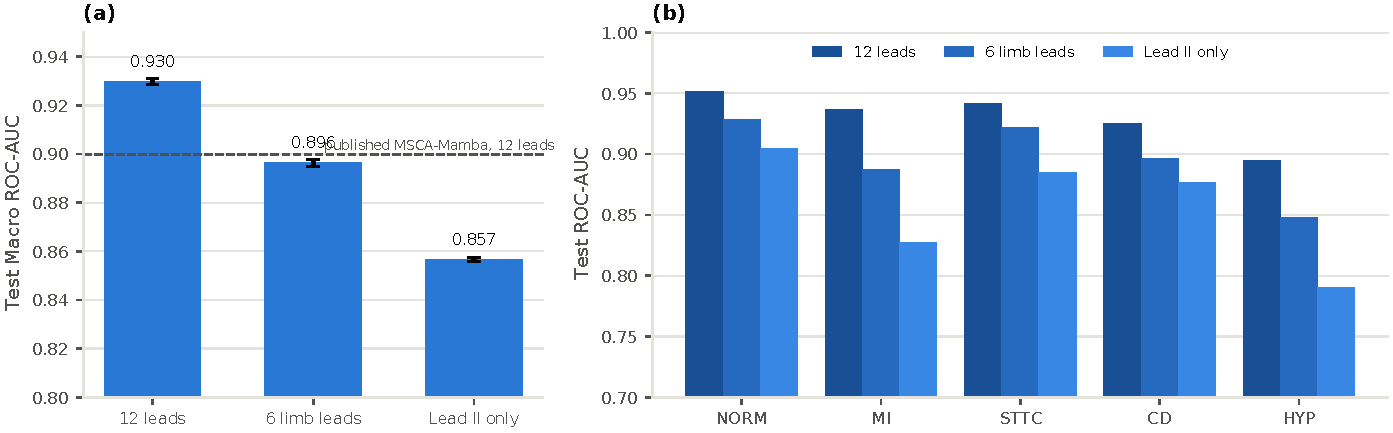
\includegraphics[width=\linewidth,height=0.36\textheight,keepaspectratio]{f21_reduced_leads.pdf}
\caption{Aggregate and classwise performance of complete twelve-lead VOLT-KD and its six-limb-lead and lead-II student variants. All configurations use twelve-lead ECGFounder soft labels. Aggregate metrics correspond to Table~10 in the main manuscript.}\label{fig:leads}
\end{figure}

\section{Ensembles, Parameter Configurations, and Local Attribution}
Table~\ref{tab:ensemble} compares single-model averages with five-seed probability ensembles. The VOLT-KD ensemble achieved macro AUC 0.9326 and AP 0.8338, above single-model averages of 0.9298 and 0.8274. Macro F1 was 0.7541 versus 0.7542, and subset accuracy was 0.6006 versus 0.6168. Ensembling mainly improved ranking, while threshold-based metrics changed in different directions. The primary configuration remains single-model deployment; ensemble results provide a reference under additional computational budget.
\begin{table}[htbp]
\centering\footnotesize
\caption{Single models and five-seed probability ensembles. Single-model rows report means and standard deviations of five independent runs; ensemble rows report one joint evaluation. Bold marks the higher result separately within single-model and ensemble groups.}\label{tab:ensemble}
\begin{tabularx}{\linewidth}{Yrrrr}
\toprule
Configuration & Macro AUC & Macro AP & Macro F1 & Subset accuracy \\
\midrule
MSCA-Mamba, Single-model mean & $0.8950\pm0.0024$ & $0.7536\pm0.0033$ & $0.6941\pm0.0021$ & $0.5618\pm0.0219$ \\
MSCA-Mamba, Five-seed ensemble & 0.9031 & 0.7713 & 0.7044 & 0.5820 \\
VOLT-KD, Single-model mean & $\boldsymbol{0.9298\pm0.0012}$ & $\boldsymbol{0.8274\pm0.0020}$ & $\boldsymbol{0.7542\pm0.0009}$ & $\boldsymbol{0.6168\pm0.0131}$ \\
VOLT-KD, Five-seed ensemble & \textbf{0.9326} & \textbf{0.8338} & \textbf{0.7541} & \textbf{0.6006} \\
\bottomrule
\end{tabularx}

\end{table}

Parameter count versus AUC reflects the combined resource trade-off of input design and structural simplification (Figure~\ref{fig:pareto}). Training counts include the relevant auxiliary branches; deployment counts appear in Table~12 in the main manuscript. Figure~\ref{fig:saliency} shows five correctly classified, high-confidence examples from complete VOLT-KD with seed 42, one per class. The sign of gradient-times-input indicates the local signal's first-order contribution direction to the current class score. These attributions provide illustrative evidence of waveform use, with interpretation restricted to the displayed records.
\begin{figure}[htbp]
\centering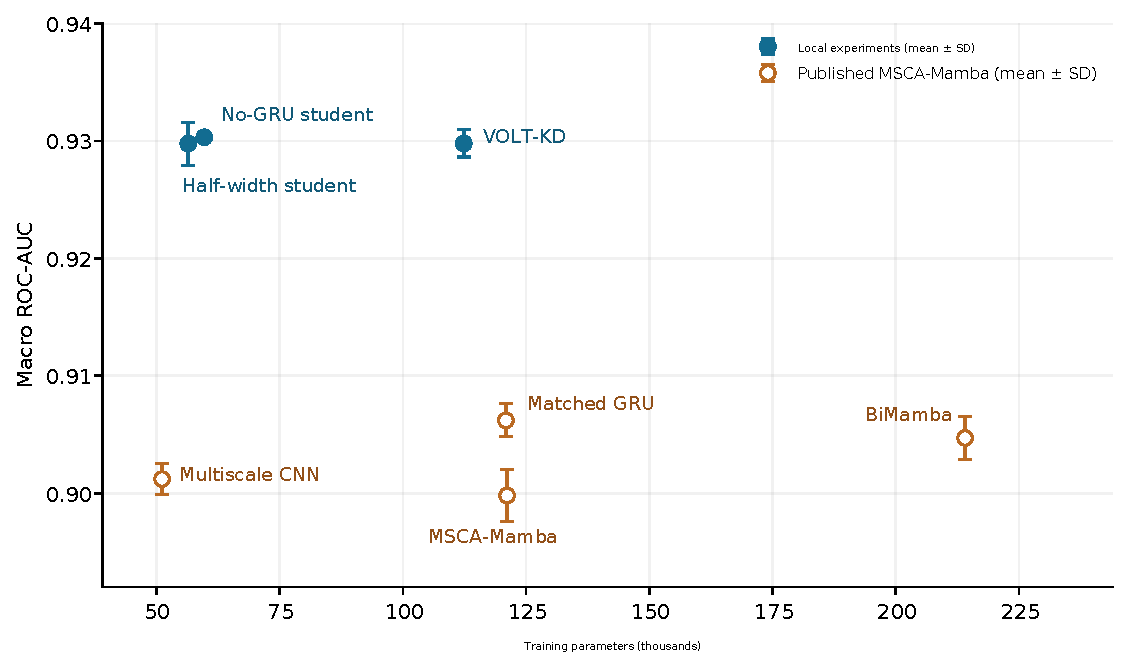
\includegraphics[width=\linewidth,height=0.45\textheight,keepaspectratio]{f14_pareto.pdf}
\caption{Training parameter counts and macro ROC-AUC of representative compact configurations. Filled points denote complete VOLT-KD, half-width, and no-GRU variants using five, three, and three seeds, respectively. Open points are configurations from the MSCA-Mamba paper\cite{cetintas2026}; remaining points are local experimental configurations.}\label{fig:pareto}
\end{figure}

\begin{figure}[htbp]
\centering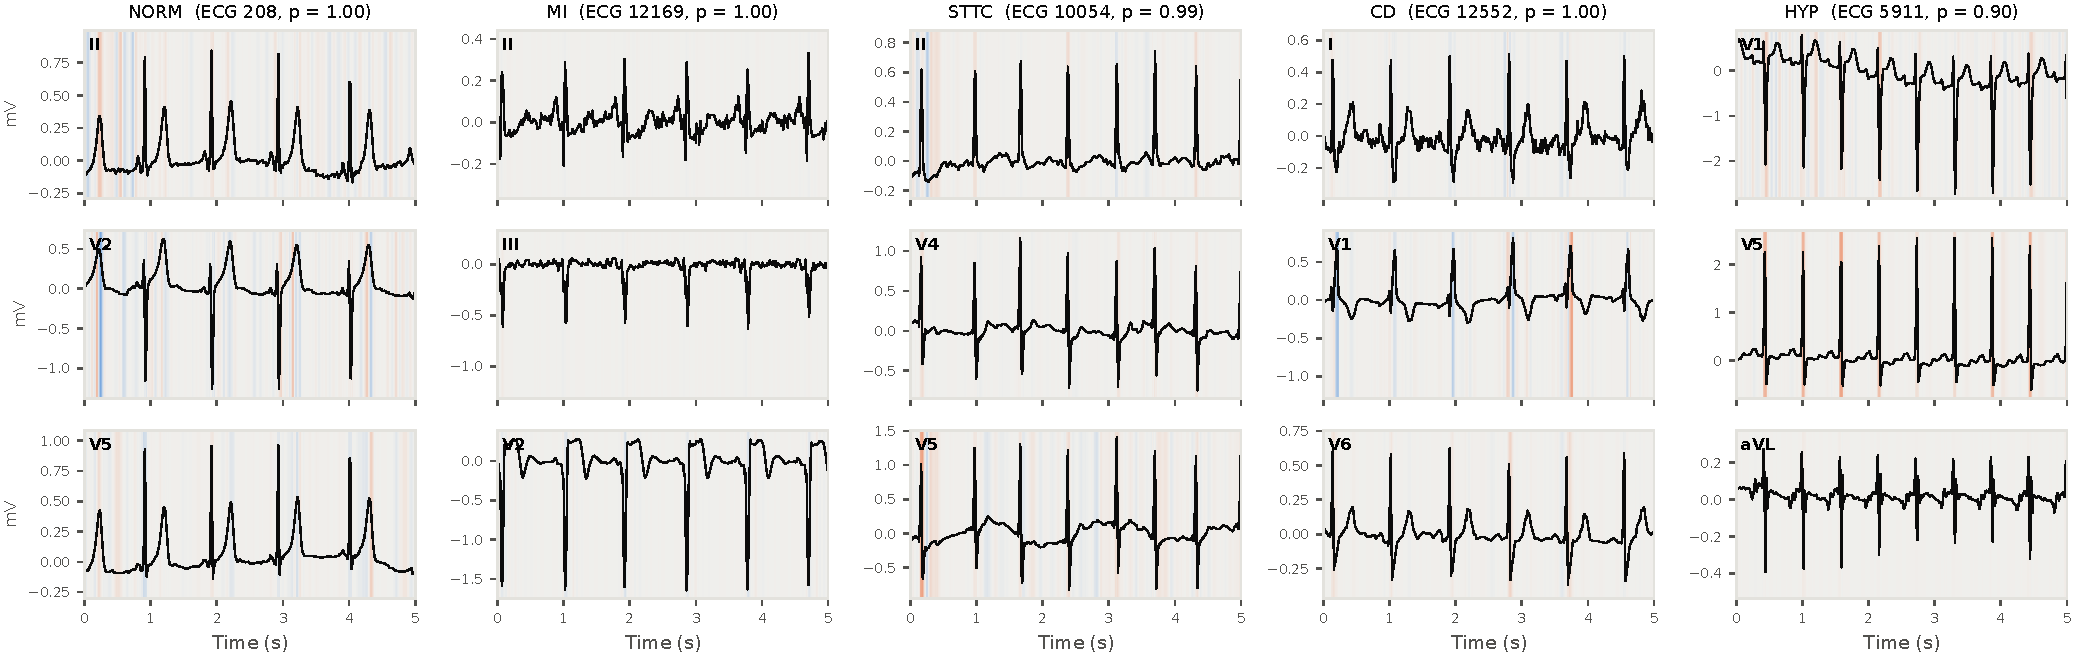
\includegraphics[width=\linewidth,height=0.72\textheight,keepaspectratio]{f23_attribution.pdf}
\caption{Gradient-times-input attributions for complete VOLT-KD. One correctly classified seed-42 test record per class is shown using three leads. Orange and blue indicate positive and negative contributions to the class score, respectively.}\label{fig:saliency}
\end{figure}

\section{Extended Literature References}
The extended comparison covers different information and computational resources (Table~\ref{tab:resource_refs}). Chimera models multivariate time series, DBA-ASFNet combines waveforms and demographics, and CNN--FFT fuses time- and frequency-domain features. Fine-tuned ECGFounder uses 500 Hz inputs, whereas heterogeneous stacking combines several inference models. VOLT-KD uses foundation-model knowledge during training and deploys one 100 Hz student with approximately one hundred thousand parameters. Differences in input information, training knowledge, and inference paths place these methods at distinct accuracy--resource trade-offs. Literature values retain the original authors' evaluation protocols.
\begin{table}[H]
\centering\footnotesize
\caption{Extended literature comparison. All external values are author-reported. Parameters are in millions (M), and bold denotes the best reported value for each metric in this table.}\label{tab:resource_refs}
\begin{tabularx}{\linewidth}{Yc p{1.65cm} rrrr}
\toprule
Method and source & Year & Input & Parameters & \shortstack{Macro\\ROC-AUC} & \shortstack{PR-AUC\\/AP} & \shortstack{Macro\\F1} \\
\midrule
Chimera\cite{behrouz2024} & 2024 & 100 Hz & -- & 0.930 & -- & -- \\
DBA-ASFNet\cite{luo2025} & 2025 & 100 Hz + age/sex & $\boldsymbol{\sim0.030}$ & 0.9166 & -- & -- \\
CNN--FFT\cite{malik2026} & 2026 & 500 Hz & 0.0869 & 0.9246 & 0.813 & \textbf{0.770} \\
Fine-tuned ECGFounder\cite{mert2026} & 2026 & 500 Hz & -- & 0.930 & 0.823 & 0.749 \\
Heterogeneous stacking\cite{mert2026} & 2026 & Ensemble & -- & \textbf{0.936} & \textbf{0.836} & 0.763 \\
VOLT-KD (ours) & -- & 100 Hz & 0.1072 & $0.9298\pm0.0012$ & $0.8274\pm0.0020$ & $0.7542\pm0.0009$ \\
\bottomrule
\end{tabularx}
\par\vspace{3pt}{\footnotesize Chimera uses the Superdiag result in Table 2 of the NeurIPS 2024 version. DBA-ASFNet uses Super-Diag. in its Table 3 and additionally receives age and sex. CNN--FFT uses its 500 Hz five-superclass results. Both Mert et al. entries come from Table I of the 2026 preprint, using official PTB-XL 1.0.3 folds and seed 42; this study reports five-seed means and standard deviations.}
\end{table}

\section{Statistical and Literature-Comparison Conventions}
Paired-seed intervals in the main text are computed as $\bar d\pm t_{0.975,n-1}s_d/\sqrt n$. HYP's arithmetic share of the macro-AUC gain is defined as $\Delta\mathrm{AUC}_{\mathrm{HYP}}/(5\Delta\mathrm{AUC}_{\mathrm{macro}})$, identifying its contribution to the equally weighted aggregate. All local checkpoints and thresholds are selected using validation data.

Literature comparisons retain the reported precision; dataset versions, inputs, and repeated-run settings appear in Table~3 in the main manuscript and Table~\ref{tab:resource_refs}. MS-LTCAF retains the source's AUC/F1 terminology, and CNN--FFT uses a 0.5 threshold.

\begingroup
\setlength{\bibsep}{3pt}
\begin{thebibliography}{99}
\bibitem{cetintas2026} Cetintas D. MSCA-Mamba: A Compact Multi-Scale Mamba Network for Multi-Label ECG Classification. \emph{Diagnostics}. 2026;16(19):3135. Published 26 September 2026. \url{https://doi.org/10.3390/diagnostics16193135}.

\bibitem{behrouz2024} Behrouz A, Santacatterina M, Zabih R. Chimera: Effectively Modeling Multivariate Time Series with 2-Dimensional State Space Models. \emph{Advances in Neural Information Processing Systems}. 2024;37:119886--119918. \url{https://proceedings.neurips.cc/paper_files/paper/2024/hash/d8e80772c27beff4ae1676fb147bbf26-Abstract-Conference.html}.

\bibitem{luo2025} Luo K, Huang L, He H, Chen Y, You L, Chen S, Chen J, Liu C. Efficient and Interpretable ECG Abnormality Detection via a Lightweight DSCR-BiGRU-Attention Network with Demographic Fusion. \emph{Mathematics}. 2025;13(23):3882. \url{https://doi.org/10.3390/math13233882}.

\bibitem{malik2026} Malik A, Aras S. A lightweight hybrid framework integrating convolutional neural networks and fast Fourier transform for reliable and calibrated ECG-based cardiac abnormality detection. \emph{PLOS One}. 2026;21(7):e0354834. \url{https://doi.org/10.1371/journal.pone.0354834}.

\bibitem{mert2026} Mert YE, Akdo\u{g}an E, \"{U}vet H. Multi-Label 12-Lead ECG Classification on the PTB-XL Dataset: A Comparative Evaluation of Deep Learning Architectures and Heterogeneous Ensemble Approaches. \emph{arXiv preprint}. 2026;arXiv:2609.12803. Posted 11 September 2026. \url{https://arxiv.org/abs/2609.12803}.
\end{thebibliography}
\endgroup

\end{document}
